\documentclass[UTF8,a4paper,11pt,fontset=fandol]{ctexart}
\usepackage[margin=18mm]{geometry}
\usepackage{amsmath,amssymb,graphicx,booktabs,hyperref,pdflscape,fancyhdr}
\hypersetup{colorlinks=true,urlcolor=blue}
\pagestyle{fancy}\fancyhf{}\fancyhead[L]{MCF：Poisson 噪声阶段对照}\fancyhead[R]{2026-10-04}\fancyfoot[C]{\thepage}
\setlength{\headheight}{15pt}\setlength{\parindent}{0pt}\setlength{\parskip}{5pt}
\begin{document}
\begin{center}{\LARGE\bfseries 圆形 MCF：散粒噪声与迭代稳定性}\par\vspace{5pt}阶段汇报\quad |\quad 呈佳伟老师\end{center}
佳伟老师：本阶段完成 48 次固定预算求解，采用有成像文献依据的探测域 Poisson 噪声；补齐 4,848 条逐步评价记录。MATLAB CPU 双精度批次用时 34.99 秒，96 项最终误差独立复核通过。
\section*{主要发现}
\begin{itemize}
\item 在两类布局、两个计数水平下，ER 的最终复场 NRMSE 均为四方法最低。$p=1$ 时周期／非周期分别为 0.6898／0.6940；$p=10$ 时为 0.2971／0.2958（三次均值）。
\item 全部 48 次求解的复场误差在 200 次传播时均高于 80 次传播。ER 的均值增幅在 $p=1$ 时为 0.1156／0.1095，在 $p=10$ 时为 0.0397／0.0390。继续迭代未改善这些含噪测量的真值误差。
\item $p=1$ 时，ER 的最终复场误差也高于初始参考（周期 0.6555、非周期 0.6739）；在四方法中最低并不等同于最终恢复优于初值。$p=10$ 时 ER 明显优于初值。
\item 原无噪声结果仍以 RAAR 最低（0.1182／0.1027）；无噪声排序不能直接推广至含噪条件。当前证据支持下一阶段研究噪声匹配与停止准则，尚未据真值选择新的停止点。请老师指导下一步重点。
\end{itemize}
\section*{本轮只改变探测噪声}
复用周期／非周期圆形端面、原 mixed 样品、支持域、已知理想参考场与固定算法参数。$2$ 布局$\times2$计数水平$\times3$种子$\times4$算法，共48次；每次200次正／反传播。无噪声结果复用原始保存记录。
\[
\alpha=\frac{p}{\langle I_{\rm ref}\rangle},\qquad
K_i\sim\operatorname{Poisson}(\alpha I_i),\qquad
A_i=\sqrt{K_i/\alpha},\quad p\in\{1,10\}.
\]
$p$ 为\textbf{空白参考帧全 $256\times256$ 像素平均检测计数}，单位为计数/像素/帧。样品吸收保留：实际期望样品均值为周期 $0.4206p$、非周期 $0.4126p$。不叠加读噪。随机种子为41001、41002、41003，同一条件下四算法共享同一输入。
\textbf{适用范围：} 单个合成样品、理想已知校准、固定参数，三次重复仅初步检查稳定性。本实验没有模拟低光子条件下参考校准的退化，不代表端到端实验系统性能。历史“20万总电子+1电子读噪”结果单独保留为工程测试。
\clearpage\begin{landscape}\thispagestyle{empty}
\section*{图1：误差随传播预算变化}
\begin{center}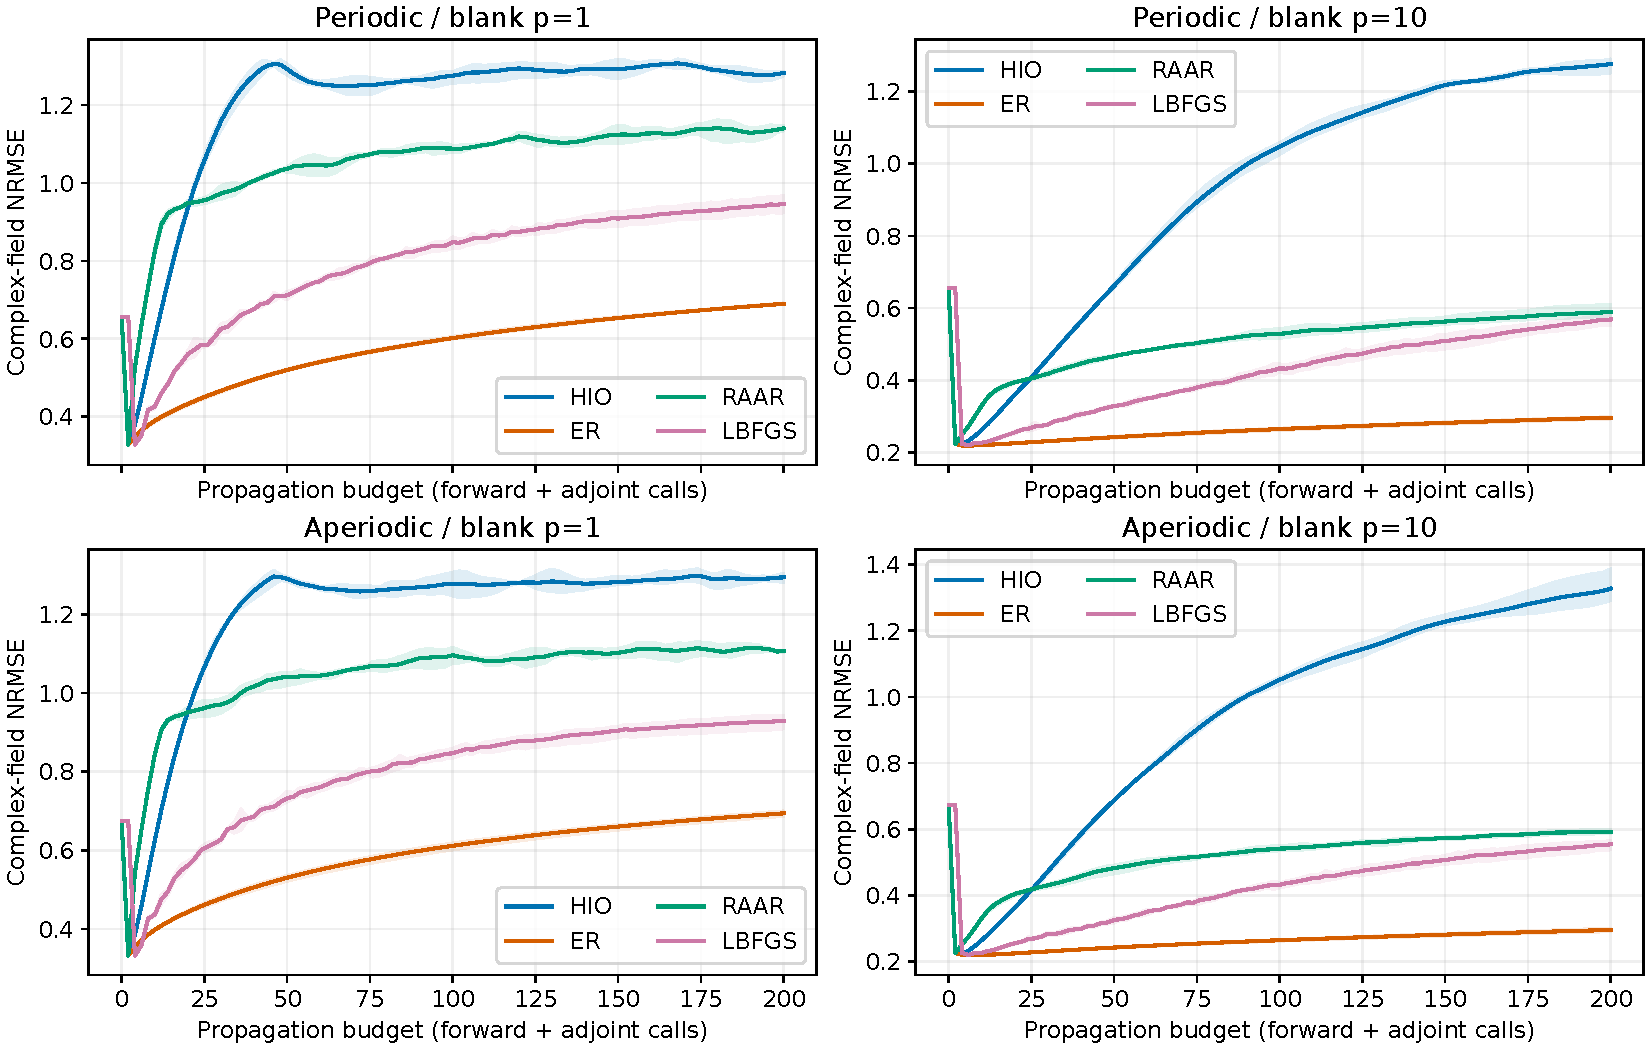
\includegraphics[width=242mm,height=143mm,keepaspectratio]{figures/convergence.pdf}\end{center}
\small 实线为三个种子的均值，阴影为最小--最大范围；四个面板对应两种布局与空白参考 $p=1/10$。本轮每2次传播记录一次，含初值，共4,848条记录，未平滑。48次均达到200次传播，无提前停止。HIO/ER/RAAR对应100次迭代；L-BFGS包含初始梯度及被拒绝线搜索的计算，横轴以实际传播开销公平比较，接受迭代数另存CSV。指标越低越好。\end{landscape}
\clearpage\begin{landscape}\thispagestyle{empty}
\section*{图2：最终误差与计数水平}
\begin{center}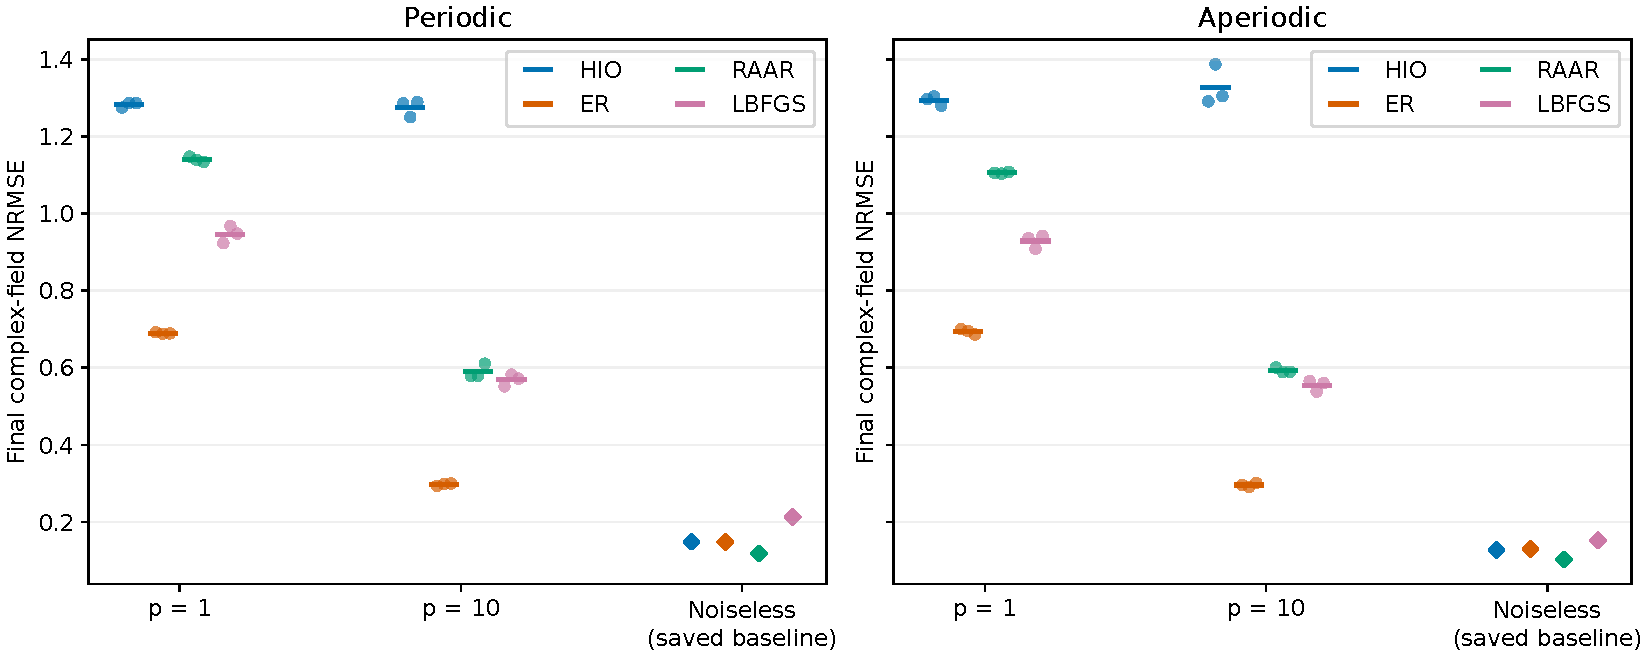
\includegraphics[width=242mm,height=140mm,keepaspectratio]{figures/noise_levels.pdf}\end{center}
\small $p=1/10$ 的圆点为各随机种子，短横线为均值；无噪声菱形为原200次传播保存结果，无新增重复。横轴是离散条件，不连接为连续光子扫描曲线。各方法均采用同一最终传播预算；相位误差及样本标准差见表1。\end{landscape}
\clearpage
\section*{表1：200次传播的最终误差}
\small\begin{center}\begin{tabular}{ll l rr}\toprule
布局 & $p$ & 方法 & 复场 NRMSE & 相位 RMSE / rad\\\midrule
周期 & 1 & HIO & $1.2828\pm0.0066$ & $1.7343\pm0.0280$\\
周期 & 1 & ER & $0.6898\pm0.0019$ & $0.6061\pm0.0154$\\
周期 & 1 & RAAR & $1.1405\pm0.0071$ & $1.5627\pm0.0208$\\
周期 & 1 & L-BFGS & $0.9464\pm0.0224$ & $1.0102\pm0.0335$\\
周期 & 10 & HIO & $1.2753\pm0.0216$ & $1.6404\pm0.0215$\\
周期 & 10 & ER & $0.2971\pm0.0032$ & $0.2066\pm0.0034$\\
周期 & 10 & RAAR & $0.5895\pm0.0183$ & $0.5013\pm0.0206$\\
周期 & 10 & L-BFGS & $0.5686\pm0.0157$ & $0.4745\pm0.0290$\\
非周期 & 1 & HIO & $1.2936\pm0.0124$ & $1.7646\pm0.0269$\\
非周期 & 1 & ER & $0.6940\pm0.0070$ & $0.5864\pm0.0073$\\
非周期 & 1 & RAAR & $1.1059\pm0.0024$ & $1.4925\pm0.0121$\\
非周期 & 1 & L-BFGS & $0.9291\pm0.0180$ & $0.9668\pm0.0295$\\
非周期 & 10 & HIO & $1.3276\pm0.0520$ & $1.7208\pm0.0649$\\
非周期 & 10 & ER & $0.2958\pm0.0053$ & $0.1985\pm0.0011$\\
非周期 & 10 & RAAR & $0.5929\pm0.0067$ & $0.4837\pm0.0079$\\
非周期 & 10 & L-BFGS & $0.5546\pm0.0145$ & $0.4455\pm0.0067$\\
\bottomrule\end{tabular}\end{center}
每项为3次重复的均值 $\pm$ 样本标准差（$n-1$分母），不作显著性检验。全部求解停止原因为达到传播预算。
\subsection*{指标与核验}
原评分ROI保持不变。令真值为 $u_\star$、共同支持域投影后的结果为 $\hat u$，仅按原ROI $\Omega$ 对齐一个全局相位：
\[
\theta=\arg\sum_{i\in\Omega}\overline{u_{\star,i}}\hat u_i,\qquad
E_u=\frac{\|e^{-\mathrm{i}\theta}\hat u-u_\star\|_2}{\|u_\star\|_2},\qquad
E_\phi=\sqrt{\frac{1}{|\Omega|}\sum_{i\in\Omega}\arg\!\left(e^{-\mathrm{i}\theta}\hat u_i\overline{u_{\star,i}}\right)^2}.
\]
复场指标在全场计算，相位指标在ROI计算；无增益拟合。真值仅用于求解后评价。17个源代码及输入哈希一致，48份完成回执校验通过，96项最终指标由保存复场独立重算。逐步曲线来自MATLAB评分记录，未另行重跑重建。
\subsection*{文献依据与迁移边界}
\begin{enumerate}\raggedright
\item \textit{Learning to synthesize: robust phase retrieval at low photon counts}, Light: Science \& Applications (2020). \newline\href{https://doi.org/10.1038/s41377-020-0267-2}{doi:10.1038/s41377-020-0267-2}，式(5)支持探测域Poisson+Gaussian形式，并研究约1/10 photons/pixel/frame。
\item \textit{Low Photon Count Phase Retrieval Using Deep Learning}, PRL (2018). \newline\href{https://doi.org/10.1103/PhysRevLett.121.243902}{doi:10.1103/PhysRevLett.121.243902}，参考照明计数定义依据。
\item \textit{Experimental robustness of Fourier Ptychography phase retrieval algorithms}, Optics Express (2015). \newline\href{https://doi.org/10.1364/OE.23.033214}{doi:10.1364/OE.23.033214}，强度Poisson鲁棒性对照依据。
\end{enumerate}
本轮选择纯Poisson分量，并以空白帧均值标定。计数水平是迁移的研究条件，未逐项复现论文探测效率、读噪或光学系统；不把检测计数直接等同于未经效率校正的入射光子数。
\end{document}
